In this section, we review the major procedures for image recognition. 
A general image recognition method consists of three parts: image preprocess, feature extraction and classification.

\begin{figure}
	\centering
	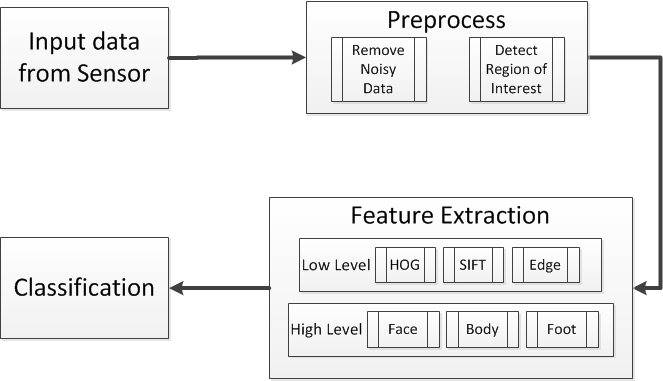
\includegraphics[scale=.8]{introduction/fig/IRflow.png}
	\caption{Major procedure for image recognition.}\label{fig:intro:irflow}
\end{figure}
\subsection{Preprocess}
The digital camera can capture the optical property of an object through its optical sensor and generate raw digital data.
After receiving the raw data of a image from the sensor, preprocess is to generate a new image from the source image. This new image is similar to the source image, but differs from it considering certain apsects, e.g. the new image has smoother edge, better contrast and less noise. 
Here, some \textit{pixel operations} and \textit{local operations} are used to improve the contrast and remove the noise.  

Another important operation of preprecess is segmentation according to the object, i.e. finding the region of interest. Images used for recognition should be aligned, making the target object appear in the central of the image and remove those irrelevant area.

The result of preprocess has great impact on the final result of the recognition. Clear and noise free images can make the feature extraction more effective and significantly improve the final classification accuracy.

\subsection{Feature Extraction}
 Feature extraction is a type of dimensionality reduction that efficiently represents interesting parts of an image as a compact feature vector. The feature vector is then used for either training the classifier or recognition. Therefore, feature extraction is the most important part for image recognition. The quality of the features extracted from a image have great impact on the recognition result. There are two major streams for feature extraction: the hand engineered method and representation learning method.
\subsubsection{Hand Engineered Feature}
Hand engineered features are typically low level and local features.
Low level features are extracted according to some optical properties of an image. These features are low level / local features. There is a widely agreement that local features are an efficient tool for object representation due to their robustness with respect to occlusion and geometrical transformations \cite{van2006coloring}. Common low level hand engineered features include Histogram of Oriented Gradients (HOG) \cite{dalal2005histograms}, Scale Invariant Feature Transform (SIFT) \cite{lowe1999object}, Speeded Up Robust Features (SURF) \cite{bay2006surf}, Local Binary Patterns (LBP) \cite{ojala2002multiresolution}, and color histograms \cite{birchfield1998elliptical}. Feature descriptors obtain from these low level features refer to a pattern or distinct structure found in an image, such as a point, edge, or small image patch. They are usually associated with an image patch that differs from its immediate surroundings by texture, color, or intensity. What the feature actually represents does not matter, just that it is distinct from its surroundings.
\begin{figure}[h]
	\centering
	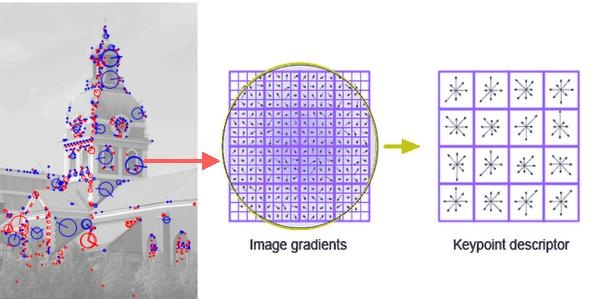
\includegraphics[scale=.6]{introduction/fig/sift.jpg}
	\caption{Feature extraction using SIFT.}\label{fig:intro:sift}
\end{figure}
These low level features can be used directly for recognition. However, since they just represent certain local properties of an image and are not discriminative enough for recognition, discriminative high level features can be further learned by combining the low level features. 

\subsubsection{Representation Learning}
Representation learning is mainly described by Deep Learning 
algorithms\cite{krizhevsky2012imagenet} or Auto Encoders\cite{bengio2007scaling}. The ideas is to learn a group of filters that are able to capture various kinds of features to discern one category of images from the another category with some supervised or unsupervised algorithm. Typically in representation learning, features are learned hierarchically from low-level features to high level ones. 
Learning representation from an image can start from either low level features (Auto Encoders) or raw pixels of an image (Deep Learning). It is generally considered that learning the good feature representations is the most important part in image recognition.
\begin{figure}
	\centering
	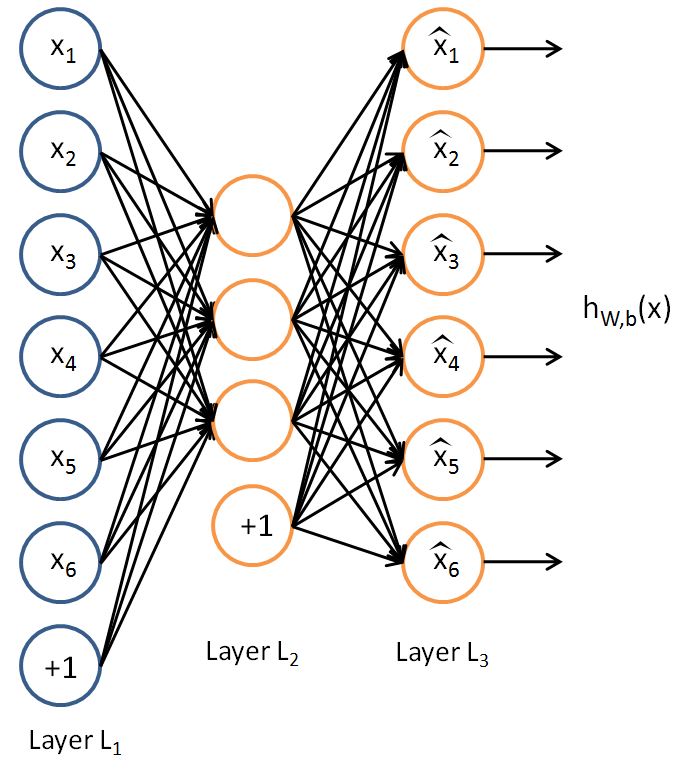
\includegraphics[scale=.3]{introduction/fig/sparsecoding.png}
	\caption{General Scheme of Auto Encoders. L1 is the input layer, possibly raw-pixel intensities. L2 is the compressed learned latent representation and L3 is the reconstruction of the given L1 layer from L2 layer. AutoEncoders tries to minimize the difference between L1 and L3 layers with some sparsity constraint.}\label{fig:intro:sparse}
\end{figure}

\textbf{Auto Encoders} are widely used to combine different types of low level feature. The outputs of the Auto Encoders are some latent representations. These latent representations are learned from the given images that have lowest possible reconstruction error. Even though the high level representations from Auto Encoders are learned by minimizing the reconstruction errors, they are still not robust enough to handle all kinds of variance of the objects.

\textbf{Deep Learning} is the most popular approach for learning representations. It has been widely used for all kinds of image recognition tasks and achieved the state-of-the-art performance on some large scale image recognition tasks, such as ILSVRC and The PASCAL Visual Object Classes Challenge (PASCAL VOC). 
Convolutional Neural Networks (CNN) is the most popular deep learning model for the image recognition tasks. The first deep CNN that had great success on image recognition is the LeNet proposed by Y.LeCan in 1989 \cite{lecun1989backpropagation}. Backpropagation was applied to Convolutional Neural networks with adaptive connections. This combination, incorporating with Max-Pooling and speeding up on graphics cards has become an important part for  many modern, competition-winning, feedforward, visual Deep Learners. Deep CNNs have been widely used as the feature extractor for all kinds of images recognition tasks and proven to be the most powerful method for feature extraction.
\begin{figure}
	\centering
	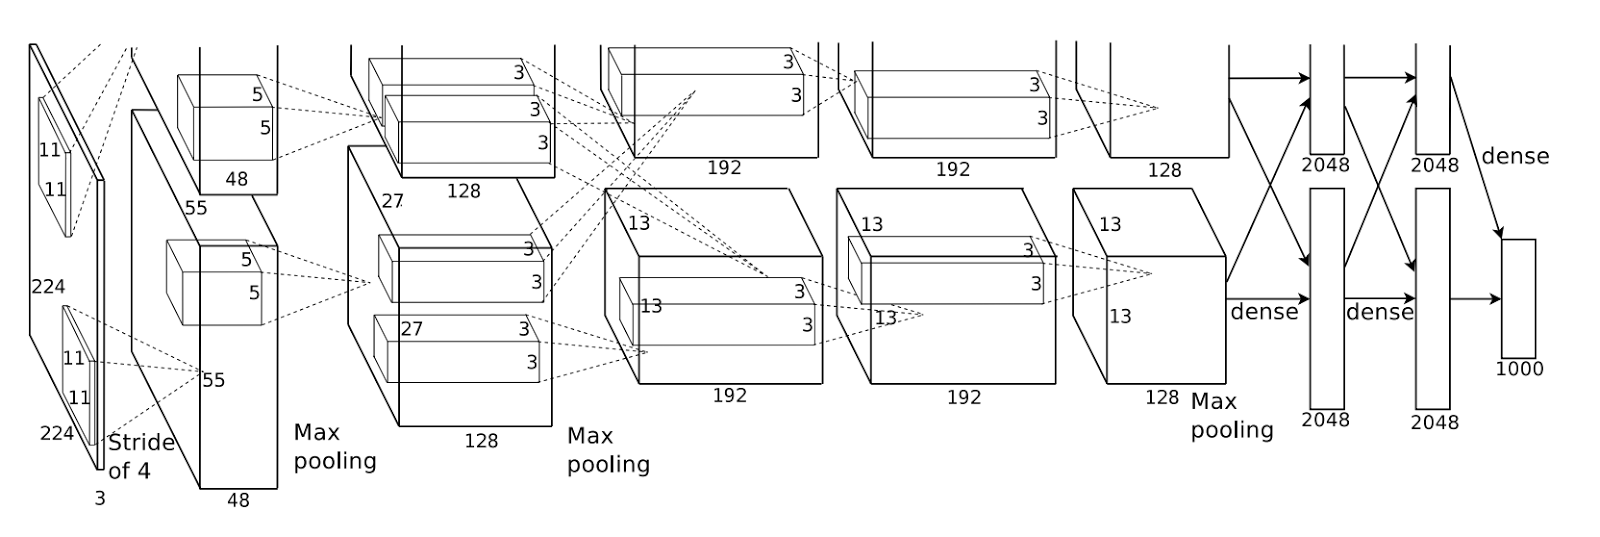
\includegraphics[scale=.3]{introduction/fig/alexnet.png}
	\caption{The architecture of ALEXNET (adapted from \cite{krizhevsky2012imagenet}).}\label{fig:intro:alex}
\end{figure}

\subsection{Classification}
After extracting feature representation from the images, a classifier should be used to train a recognition model as well as for predicting the new coming images. A supervised model is always used for training the recognition model. Discriminative classifier such as Support Vector Machine (SVM) is widely used as the classifier for recognition \cite{cristianini2000introduction}. As we mentioned before, in order to capture different variances of the images for one category, the size of the feature representation for a image is usually very large. In order to avoid overfitting, the size of the training set should be at least the same size of the size of the feature representation as well. Some classifiers such as Bayesian method or decision tree require to consider the correlations between each feature and the class labels and suffer from the large feature dimension. However, Discriminative model are more convenient for training and can be effectively optimized with stochastic gradient descent which is suitable for very large training set \cite{bottou2010large}.

In this thesis, we focus on how to transfer the knowledge from the source domain to the target domain. The methods proposed for VTL are mainly focus on the stage of classification, i.e. how to build classifier to leverage the source knowledge when we can only visit the source model.



